\newpage
\section{Durchführung}
    \subsection{Versuchsaufbau}
        \begin{figure}[h]
          \centering
          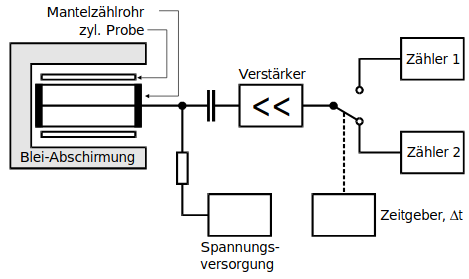
\includegraphics[width = 0.6\textwidth]{pictures/Aufbau.png}
          \caption{Hier ist der Aufbau der Versuchsschaltung dargestellt.}
          \label{fig:Aufbau}
        \end{figure}

        \FloatBarrier

        An den Szintillator sind zwei Photomultiplier (PMT) angeschlossen, um mögliche Störungen, die an nur einem PMT in die Messung einfließen können mithilfe der Koinzidenz auszuschließen.
        Damit die Signale möglichst zeitgleich an der Koinzidenz ankommen werden hinter die PMTs Verzörgerungsleitungen, die aus Kabelspulen bestehen, dazugeschaltet.
        Die Diskriminatoren filtern je nach eingestellter Schwelle Signale.
        Wie schon erwähnt lässt die Koinzidenz nur ein Signal durch, wenn alle Input-Signale in einer bestimmten Auflösungszeit ankommen.

        Anschließend ist eine, durch eine elektronische Schaltung realisierte, Stoppuhr aufgebaut. Die Koinzidenz ist über eine weitere Verzörgerungsleitung und eine monostabile Kippstufe (Monoflop) an zwei AND-Gatter angeschlossen. Diese sind mit einem Time-Amplitude-Converter (TAC) verbunden, welcher selbst an einen Vielkanalanalysator (Multi-Channel-Analyser, MCA) angeschlossen ist. Ein Computer liest diesen aus und speichert die gemessenen Daten.

    \subsection{Wirkungsweise der "Stoppuhr-Schaltung"}
        Zuerst wird die Funktionsweise eines Monoflop beschrieben: \\
        Solange er nicht getriggert wird, gibt er ein Signal aus seinem negativen Output aus.
        Wird der Monoflop getriggert wird das gesendete Signal über einen eingestellten Zeittraum, die Suchzeit $T_{\text{S}}$, vom negativen zum positiven Output gewechselt. Während dieser Suchzeit bewirken ankommende Signale nichts am Monoflop.

        Das erste AND-Gatter bekommt das Signal der Koinzidenz als auch das negative Signal des Monoflop als Input.
        Das heißt

        Die Koinzidenz gibt ein erstes Signal aus. Dieses erreicht einerseits das 1. AND-Gatter als auch mit einer Verzörgerung von $30$ns den Monoflop, der 

    \subsection{Halbwertszeitbestimmung von Vanadium}
        Zur Halbwertszeitbestimmung von Vanadium wird eine Vanadiumprobe zunächst an einer Neutronenquelle platziert. Nachdem diese dort aktiviert wurde, wird sie in dem Zählrohr platziert und 
        die Aktivität über ein Messintervall von 30 Sekunden gemessen. Alle 30 Sekunden wechselt der Zeitschalter auf den anderen der zwei Zähler und ermöglicht so ein Ablesen der Zählrate auf
        dem anderen Zähler.

    \subsection{Halbwertszeitbestimmung von Rhodium}
        Die Rhodiumprobe wird entsprechend der Vorbereitung der Vanadiumprobe auch neben der Neutronenquelle aktiviert. Die Messung der Aktivität verläuft analog zur Messung der Vanadiumprobe
        mit einer Messzeit von 15 Sekunden. Auch hier ermöglicht der Zeitschalter ein kontinuierliches Messen.
        
